\documentclass[a4paper, 11pt]{article}

\usepackage[ mincrossrefs=999, style=numeric, backend=biber, url=false,
isbn=false, doi=false, ]{biblatex}

\addbibresource{references.bib}

\usepackage[margin=1in]{geometry} \usepackage[dvipsnames]{xcolor}
\usepackage[colorlinks]{hyperref} \usepackage{enumitem} \usepackage{amsfonts}

\usepackage{unicode-math}
\usepackage{stmaryrd}
\usepackage{amsfonts}
\usepackage{mathtools}
\usepackage{xspace}

\NewDocumentCommand{\codeword}{v}{%
\texttt{\textcolor{gray}{#1}}%
}

\NewDocumentCommand{\term}{v}{%
\texttt{\textcolor{blue}{#1}}%
}
\NewDocumentCommand{\keyword}{v}{%
\texttt{\textcolor{orange}{#1}}%
}

\usepackage{ stmaryrd }

% \usepackage{enumitem}
\setlist[itemize]{noitemsep, topsep=0pt}

\hypersetup{ citecolor=RoyalBlue }

\usepackage{fontspec}

\usepackage{titlesec}

\titlespacing\section{0pt}{4pt plus 2pt minus 2pt}{4pt plus 2pt minus 2pt}

\usepackage{graphicx} % for images
\usepackage{float} % for figure[H]

% \setmainfont{Linux Libertine} % \setsansfont{Linux Biolinum} % %
% \setmonofont[Scale=0.85]{PragmataPro Mono Liga}

\begin{document} \pagenumbering{gobble}

\begin{titlepage}

\vspace*{1cm}

\begin{center} \Large Notions of syntax and semantics
  for voice assistants in autonomous vehicles  \\ 

% gurantess robustness? 
% autonomous vehicles ?

\vspace{1.5cm}

\large Warrick Macmillan  \\
\large Developed with the support of Ekaterina Komendantskaya
\end{center}


\end{titlepage}

\section{Abstract} 

We introduce a grammar for a controlled natural language (CNL) to give
imperative commands to an envisioned voice assistant for a self-driving car. The
utility of the CNL is that it is inductively defined as a grammar : thereby, the
sentences it admits, parsed as Abstract Syntax Trees (ASTs), can be manipulated as
mathematical objects amenable to verification techniques. Using the TOUCHDOWN
data set to motivate common idioms and phrases our grammar should be capable of
parsing, we give a denotational semantics to a subset of Linear Temporal Logic
formulas, essentially expressing sequences of states, which are 
amenable as specifications to downstream applications whose goal is the
verification of various aspects of a vehicles behavior. We see this work 
as a preliminary contribution to a large literature as regards CNLs,
verification for natural language-controlled robots, and semantic parsing.

\section{Contributions}

Initially motivated to give the system assurances against so-called
substitution-based attacks, whereby synonyms can be given the same meaning by
imposing posterior conditions on the parse trees. Clustering over the tree
structure to provide some kind of equivalence to meaningfully similar sentences
was an initially enticing direction, as had been done with Komendantskaya and
Heras' work on Machine Learning for Proof General (ML4PG) \cite{ml4pg}. However,
this work had the advantage that there are multiple large, well-maintained Coq
libraries which were amenable to clustering, whereby successful results could
give rise to use in downstream applications.

Our use case being the design of a non-existent language left us with the
conundrum of an impoverished data set to train over and the issue of what
utility this would be for downstream applications. What followed may then be
seen as a response to these constraints : find a data set suitable to give
examples of non-trivial natural language utterances, in addition to finding a
suitable semantic language with utility and applicability which is amenable to
translation from sentences parsed by our grammar.

The primary contributions during this project are as follows :

\begin{itemize}[noitemsep]
\item A Grammatical Framework (GF) grammar providing the definition of a CNL for
directives to a driving agent
\item A Haskell mapping trees of our grammar a particularly well-behaved subset of LTL
\item An Agda implementation of LTL with a standard semantic interpretation
\item A refinement of the TOUCHDOWN dataset \cite{chen2019touchdown}, suited to our needs of designing a
better grammar
\end{itemize}

We suggest that while each of these components are still relatively primitive,
they define a pipeline which has potential to provide both theoretical insights
to researchers and suggest possible practical steps that can be taken to
building robust voice applications in industrial settings. In addition to
discussing our own contributions, we try to give a comprehensive literature
review that embeds our work in the context of interesting ongoing work happening
around the world.

\section{Overview}

Perhaps the most pervasive question in the use and application of natural
language technologies, and one which exemplifies the boundary of the
``formalist'', verification-minded and ``empiricist'', data-oriented camps in
designing such technologies, can be stated as follows : How does one optimize
the system to provide for wide coverage of the domain while ensuring that system
is robust?

The statistical and machine learning methods applied to Natural Language
Processing tasks have made enormous gains over the past three decades. They take
a more pragmatic approach : compromise robustness for wide coverage, as this
means the tools will be usable and by non-experts, where many believe that the
machines should ``learn'' from us. Somewhat orthogonal, the formal approaches in
computational linguistics, instead, are often more concerned with theoretical
justification and explainability. While practical tools are a goal, their
practical applications often aren't linguistically informative and therefore
they shouldn't override work on building the theoretical models which enable our
understanding of the machines. The developers of these theoretically informed
systems seek predictable and well-defined behavior for specific problem domains.
Yet, these systems fail to generalize without an explosion in complexity when
presented with data outside their domain.

Natural language both is structured with respect to rules, admitting lots of
predictability, yet continuously breaks or introduces exceptions to these rules.
This makes it exceedingly hard to penetrate from exclusively the empirical or
formalist approach. This leads many to wonder about the degree to which large
amounts of data can be augmented with theoretical knowledge about natural
language to create optimal and practical systems with respect to both breadth
and depth of coverage of language phenomena. The ultimate question seeking
compromise from both camps asks : how can we build machines which ``understand'' us
(or at least our data), and which allow us to understand them.

This problem acutely arises in when trying to design a voice assistant in the
domain of commanding controllable robots, specifically, autonomous vehicles. For
the actions a vehicle takes, mostly the motion and path decisions, must be
formally specified or at the very least controlled via some computer system
subject to mathematical formalism. Assuming the user directing the vehicle isn't
aware of these formalisms, it is incredibly difficult to design a verifiable
controller capable of dealing with the breadth of language one may encounter in
the wild.

The instructions an arbitrary user gives are not subject to the same formalities
the system requires. For her commands may leave out detail (``go into the other
lane'' with multiple lanes on either side), say something wrong with respect to
reality (``go into the other lane'' on a single lane road), or give a command
the controller should recognize as possible but bad (``drive directly into the
car ahead''). Additionally, the controller may need to recognize many ways many
users may say ``the same thing'', that is the same with respect to some semantic
formalism. It is obviously worrisome that a nefarious actor may somehow
interfere with the controls at any stage, particularly the point at which a
linguistic utterance is made, and reassuring one this doesn't happen is critical
for such technologies to see adoption.

We therefore analyze our ``big-picture'' question above in the following
``sub-question'' : how can one map the manifold ways of presenting information to an
autonomous robot into a rigorous and formally verifiable kernel which the
controller can understand? Our proposed solution is to build a semantic parser
from natural language commands to Linear Temporal Logic (LTL), whereby we can filter
the many possible natural language commands into a ``canonical subset'' which
are equivalent to (sets of) temporal logic formulas. We detail here both the
progress to these ends, as well as the challenges.

\section{Previous Work} 

This research broaches many different research fields, many of which were
unknown to the author prior to this work. Indeed, voice assistants can
encompass almost any natural language processing task, autonomous vehicles are
one of the premier emerging robotics technologies (and certainly the most talked
about in the media), and the cyberphysical systems at their intersection is
likewise incredibly broad.

Limiting the scope of work in this context can be challenging, as so many
different tools and ideas can be seen as relevant. We therefore try to very
explicitly narrow our focus to investigate how feasible it is to build a
language for an autonomous vehicle that exhibits predictable behavior but also
satisfies verification properties (and to determine to what extent the
properties can even be stated).

The approach taken therefore sets out to build a semantic parser, even if
primitive, that serves as a Petri dish through which many of the deeper questions
in this space may be viewed.

\subsection{GF, Parsers, and Personal Work}

The questions of designing a suitable formal language, with roots in Frege
\cite{frege79}, manifested more recently in the natural language semantics of
Montague \cite{Montague1973}, who proposed an interpretation of English in a
typed higher order logic with a focus on quantifiers. Aarne Ranta, a student of
Martin-Löf, attempted to reformulate Montague's work in an intuitionistic
setting \cite{ranta1994type}. In implementing a parser from natural language to
a dependent type theory, Ranta discovered that dual sugaring (or pretty
printing) transformation of a formal tree to a string way of going could allow
for a general mechanism of purely syntax-based translation. This work culminated
in Grammatical Framework (GF) \cite{ranta_2004}.

Grammatical Framework became a full research project, allowing for the simple
specification of a parser using a statically typed programming language whereby
the grammar rules could be seen as types, and separate concrete syntax's
cohering with a given abstract syntax allowed for language-specific parsing. The
GF ``standard library'', the Resource Grammar Library (RGL) \cite{ranta2009rgl},
allows one to get off-the-shelf grammatical constructions for more than 30
languages, with English being the most comprehensive. The RGL therefore allows
the grammar writer to focus on the semantic domain of the application the
grammar is being developed for. In addition to this, one can embed grammar
abstract syntax as Generalized Algebraic Datatypes (GADTs) in Haskell via the
Portable Grammar Format (PGF) \cite{angelov2010pgf}, whereby one can get
run-time support for parsing and linearization, in addition to manipulating the
trees by pattern matching over them as Haskell programs.

A reflection on these historical developments reveals that GF is intimately tied
to both the formal/informal distinction, in addition to the syntactical and
semantical approaches in computational linguistics. These dual characteristics
very much inform out problem as well. In the context of designing a voice
assistant for an autonomous vehicle, whereby one can give commands like ``turn
right after the woman with the big dog'', we desire that the intensional belief a
user has about her utterance is consistent with the extensional behavior of the
vehicle. This can be done through an intermediary mapping to a formal semantic
representation. Ensuring that the syntactic content of a voice director's
(well-formed) utterance maps predictably to the logical form is important from
the verificationist perspective : one wants to maximize the \emph{syntactic
completeness} of the system \cite{macmillan2021}.

In a dual situation which we don't address but briefly mention, we can imagine
our voice assistant as giving the user feedback, responding with clarifications
(``we will turn after the big cafe even though the other route may have less
traffic''), questions (``do you mean this or that person?''), or even possible
illocutionary directives (``we won't drive over the speed limit in a school
zone''), requires the computer to generate an utterance after it has made some
internal determination. We can vaguely consider this internal deliberation to
be a program, possibly inside or outside our semantical space, like
having identified multiple routes, or multiple possible states in the situation
with two people, or constraints based off external circumstances. In each case,
the formation of a natural language utterance requires the computer to generate
natural language which must conform to both the programs structure, but also be
clear and recognizable to the user. Independently of how the robot determines a
program whose meaning it needs to convey to a user, the property of providing a
natural language utterance which fluently conveys meaning to a native speaker is
called \emph{semantic adequacy}. Determining a reasonable syntax and semantics
for a controlled natural language should most certainly conform to both
standards of syntactic completeness and semantic adequacy, if the voice assistant
is to be held to any kind of regulatable standard.

\subsection{Semantical Representations}

\subsubsection{Robot Motion Planning}

The challenge of designing a system which generates robot control strategies
from human language has to balance the expressiveness of task specification,
complexity of environment, and provable correctness \cite{4141034}. In this
context, we assume that expressivity of the language itself should reflect the
complexity of the environments, thereby being adequately descriptive. The
correctness has two facets in here : that the language itself is
well-represented in the LTL semantics - the system is syntactically complete -
and that is the focus of these investigations.

Just as important, but not explored is here, is that the evaluation of a formula
in one's semantic domain gives a faithful solution to navigating a complex
environment. For instance, in \cite{plaku2016motion} the authors indicate how to
actually ground basic propositions from the language to paths in a space, while
our model, outputting formulas un-grounded base predicates, is merely concerned
with the logical structure.

Similarly, in \cite{7759412}, the authors develop a Verifiable Distributed
Correspondence Graph (V-DCG) model whereby LTL formulas are used to ensure
grounded instruction sequences are consistent. This work builds on other work of
Kress-Gazit's \cite{provCorrectNatControl}, whereby the The Situated Language
Understanding Robot Platform (SLURP) allows translation of arbitrary natural
language into LTL - with less reliance on grammar formalisms - and also supports
.

Our GF implementation differentiates itself from these programs in that it sees
the grammar as a necessary part of the verifiability (in that we can
systematically map our sequences of commands to logical formulas representing
sequences of states) in a way that's easy to support multi-linguality (which our
system does not support, but can easily be adjusted to so with the help of the
RGL). The lack of wide-coverage support of our grammar is possible to remediate
through possible fine-tuning of a large language model to a data-set which
coheres to the language our GF grammar generates, and we detail this in our
discussion below [TODO : link].

--
In \cite{kuo2020deep}, the authors do the most general end-to-end task without
intermediary states, namely, map natural language commands to navigation and
manipulation tasks. While this ``cutting out the middle man'' mentality may be
an idealistic long-term vision, it makes the system much too much of a black box
- for the fine-tuned verification conditions we desire to express and impose via
the intermediate symbolic representations, the intermediate states, we imagine
give us a more explainable, predictable, and regulatable system

% There is a group at MIT (Kuo, Katz, Barbu, ..) doing seemingly similar things to
% Tellex's group.

\begin{itemize}
\item

\item More similar to Tellex et al's approach \cite{patellearning},
  \cite{ltlSemParse} seek to train a model via images in a simulated world.
  Their work also uses a SCFG (to generate semantically inadequate sentences
  with corresponding LTL formulas) from which they can direct machines to
  follow the instructions, and then have users describe the instructions in more
  natural form. 
\item One of the 
\end{itemize}

\subsubsection{Temporal Logic for NL verification}

Modal logics, specifically those dealing with stateful staging of events like
Linear Temporal Logic (LTL), Computation Tree Logic (CTL), Signal Temporal Logic
(STL), have been used extensively in the specification and verification of properties
of robotics systems, including autonomous vehicles \cite{}.

With verification being a core motivation of our work, we take for granted that
these different logics have differing interpretations, utilities, or
manifestations in their different applied settings. As LTL is often seen as one
of the ``primitive'' temporal logic, we chose it as a our semantic space despite
its limitations. We appreciate that future work will need to expand the scope of 
which logic (or possibly \emph{logics}) the machine may use to verify behavior,
in addition to the mathematical models most amenable to verification of a logical formula.

We recognize that there are many degrees of freedom in the both the syntactic
and semantic formalisms chosen, as well as their evaluation or grounding within
physical environments.

\begin{itemize}
\item Parsing formalisms - phrase-based grammars (GF), categorial grammars, or
  even perhaps dependency grammars for wide-coverage usage
\item Semantic formalisms including spatial logics and vector space semantics
\item Mechanisms for evaluating and syntactic and semantic choices 
\item Robotics domains outside of the autonomous vehicle space, for which
  natural language is still an ideal interface. Ideally we'd like one system to
  be generally applicable to many areas, independent of certain nuances in a
  given space
\end{itemize}

\subsubsection{NL to TL}

Here we show mainly relevant research for NL to LTL.

The applications of LTL in machine learning are vast, and the scope of our
specific application is still unclear, but nevertheless, we give a literature
review of methods and applications relevant for our work.

\begin{itemize}

\item This paper \cite{5152776} from 2009 uses a categorial grammar approach, but more or less
  can serve as an idea template for us, also nice pictures with grammar rules
  and formulas
\item Also, a highly relevant template combines Natural Language, LTL, with the
  idea of having a verifiable pipeline \cite{provCorrectNatControl} 

\begin{quote}
The production of an on-
tology of common actions and the type of formulas that
they produce—for example, safety conditions, adding goals,
constraining the initial state—in their negated and positive
forms would be a step toward a more general solution to
the problem of mapping natural language to LTL. Previous
work has relied heavily on grammar formalisms to ease...
\cite{provCorrectNatControl} 
\end{quote}

\item LTL formulas can be transformed into automata which can then be used as reward functions for reinforcement learners, as in \cite{ltlRein}

\item  The following is one of the more relevant quotes from a paper reviewing
  the whole space of English to LTL translations
  \begin{quote}
Overall, the typical approach followed by these studies can be summarized as follows:
given an input English utterance, preprocess it to extract syntactical information, which may
include part of speech tagging, dependency parsing, semantic role labelling, and so on. Then,
enrich the input with these pieces of information. Finally, run an attribute grammar-based
parser, or rely on some hand-made rules, to derive a translation into a target logical format.
A notable exception is the work of [89], where a fully-supervised learning setting is considered.
\cite{brunello_et_al}
\end{quote}
\item Translating between English and STL can be done via a large language model 
\cite{he2021english} [under review], but the domain specificity of the problems
are still significant enough to suggest that it will be years before an
automated semantic parser is available, if it is even possible. 
\item Could ask Lapata in Edinburgh, whose work \cite{dong-lapata-2016-language}
  is relevant and well-cited (although they use an encoder-decoder method)
\item
\item
\item

\end{itemize}

\subsubsection{Tellex}

Stephanie Tellex has written extensively about natural language inputs and
interfaces with robots. Although she has not specifically written about
autonomous vehicles, the domains have enough intersection to warrant careful
consideration of much of her work, especially the recent stuff.

\begin{itemize}

\item Grounding with an intermediate symbolic state, no LTL, but possibly
  relevant for paper generally. She also cites \cite{walkTalk}, a seminal paper in this area
\begin{quote}
Instruction following is a supervised learning problem
where the agent must predict a trajectory that would satisfy an
input natural language command. \cite{tellexInstr}
\end{quote}
\item The review paper \cite{MARGE2022101255} making recommendations has a
  section on robustness, but this is mostly for the sake of allowing sharing of
  interfaces and efficacy, no mention of verification (which is what we're
  primarily after)
\item They design a NL -> LTL for drones that are grounded to actual landmarks \cite{9197068}
\item The group builds a trained pipeline that uses an object oriented
  template-instance methodology to generalize to different ontological
  categories in  \cite{hsiung2021generalizing} [under review]

\item In \cite{patellearning} build learn a semantic parser from NL to LTL (so
that the language is grounded) where they collect executions of the LTL formulas
in different environments using a weakly-supervised training method with
reinforcement learning Part if the paper has to do with the execution of the
command being dependent on the path taken by the robot executing the command,
not just meeting the goal requirements, thereby giving a complexity bonus in
comparison to previous work. She also evaluates the model on the \cite{walkTalk}
data set
\end{itemize}



\section{Work} 

\subsection{GF Grammar}

\section{TODO} 

\subsection{Grammar modulo wordnet}

\subsection{LTL in Agda}

Along with colleagues from Singapore Management University, we have begun an
Agda implementation \cite{wltl} of LTL which will serve as the semantic space
for our parsed utterances. Our method, uses a deep embedding, as opposed to the
shallow embedding in \cite{coqLTL}, although the temporal encoding of paths as
streams was directly adapted from this paper.

This implementation will hopefully allow us to prove decidability of LTL in a
relatively straightforward manner. Other than the assurance that our
implementation is correct, we hope this will allow us to feed the formula into
some SAT or SMT solver so-as to actually allow verification of the behavior of a
vehicle with respect to an utterance.

[TODO : Help from Matthew?]

\subsection{AST -> Agda}

\subsection{ML training/verification stuff}
Help from Marco, Nathalia if interested?


\section{Publications Description}

Realizing that the structure of the paper is ameanable to large changes, I'm
posting a summary of relevant publications here.

\subsection{Statistical (pre-trained) Language Models}
The first set of publ

\begin{itemize}

\item In \cite{fewShotSem} [under review], the authors show how, using a \emph{synchronous
context-free grammar} (SCFG) to define a minified CNL with a parallel and dually
parsible semantic form, that one can use a large pre-trained language model as a front-end
to filter a much wider syntax into the CNL. I postulate GF's expressivity is
more expressive than the SCFG, at least based off a tertiary reading in the
index, and therefore if we carved out a subset of commands to cohere with our
LTL (and maybe some other temporal or even spatial-temporal logics in the
future), our model would be amenable to a similar ``out-of-the box" semantic
parser that could actually be used for verification. This paper borrows the idea
of ``semantic parsing as paraphrasing'' from  \cite{berant-liang-2014-semantic}

\item In \cite{dontParse}, the authors advocate for getting rid of parsers
  alltogether, although this naively takes for granted large public data-sets,
  none of which exist for an autonomous vehicle and temporal logic formalism
\item  \cite{hauser2021bert} [under review] claims that Bert is robust, analyzing claims of four
  papers, including the one which uses a wordnet attack

\end{itemize}

\subsection{Voice assistants for autonomous vehicles}

The public company Cerence \cite{} is already designing voice assistants for autonomous
vehicles, for which it has a large software stack between the voice processing
to actual control of current automative components. In addition to its 
technologies, many of which aren't accessible to external researchers due to
intellectual property restrictions, Cerence has contracts with large automakers
[..]. It is therefore natural to inquire, what a small team with varied
backgrounds and not nearly the same expertise nor experience within the
technological team at Cerence can provide.

First, we believe that the focus on verification, insofar as we envision it, is
unlikely to be of current concern at Cerence due to the fact that their products
are still being developed, and the primary goal of producing a working product
is likely to precedence over preventing non-existent hostile actors.

Additionally, it is going to have to be determined by 
[verification of self-driving cars generally : software, hardware, behavior in
a real environment, etc]



\section{Future Work}

The ``sets of'' clause
references the inevitable ambiguity of parses even from a big enough parser, even
if the size of the canoncial expressions is vastly smaller than the domain of
expressions mapping to them.

\begin{figure}[H]
\centering
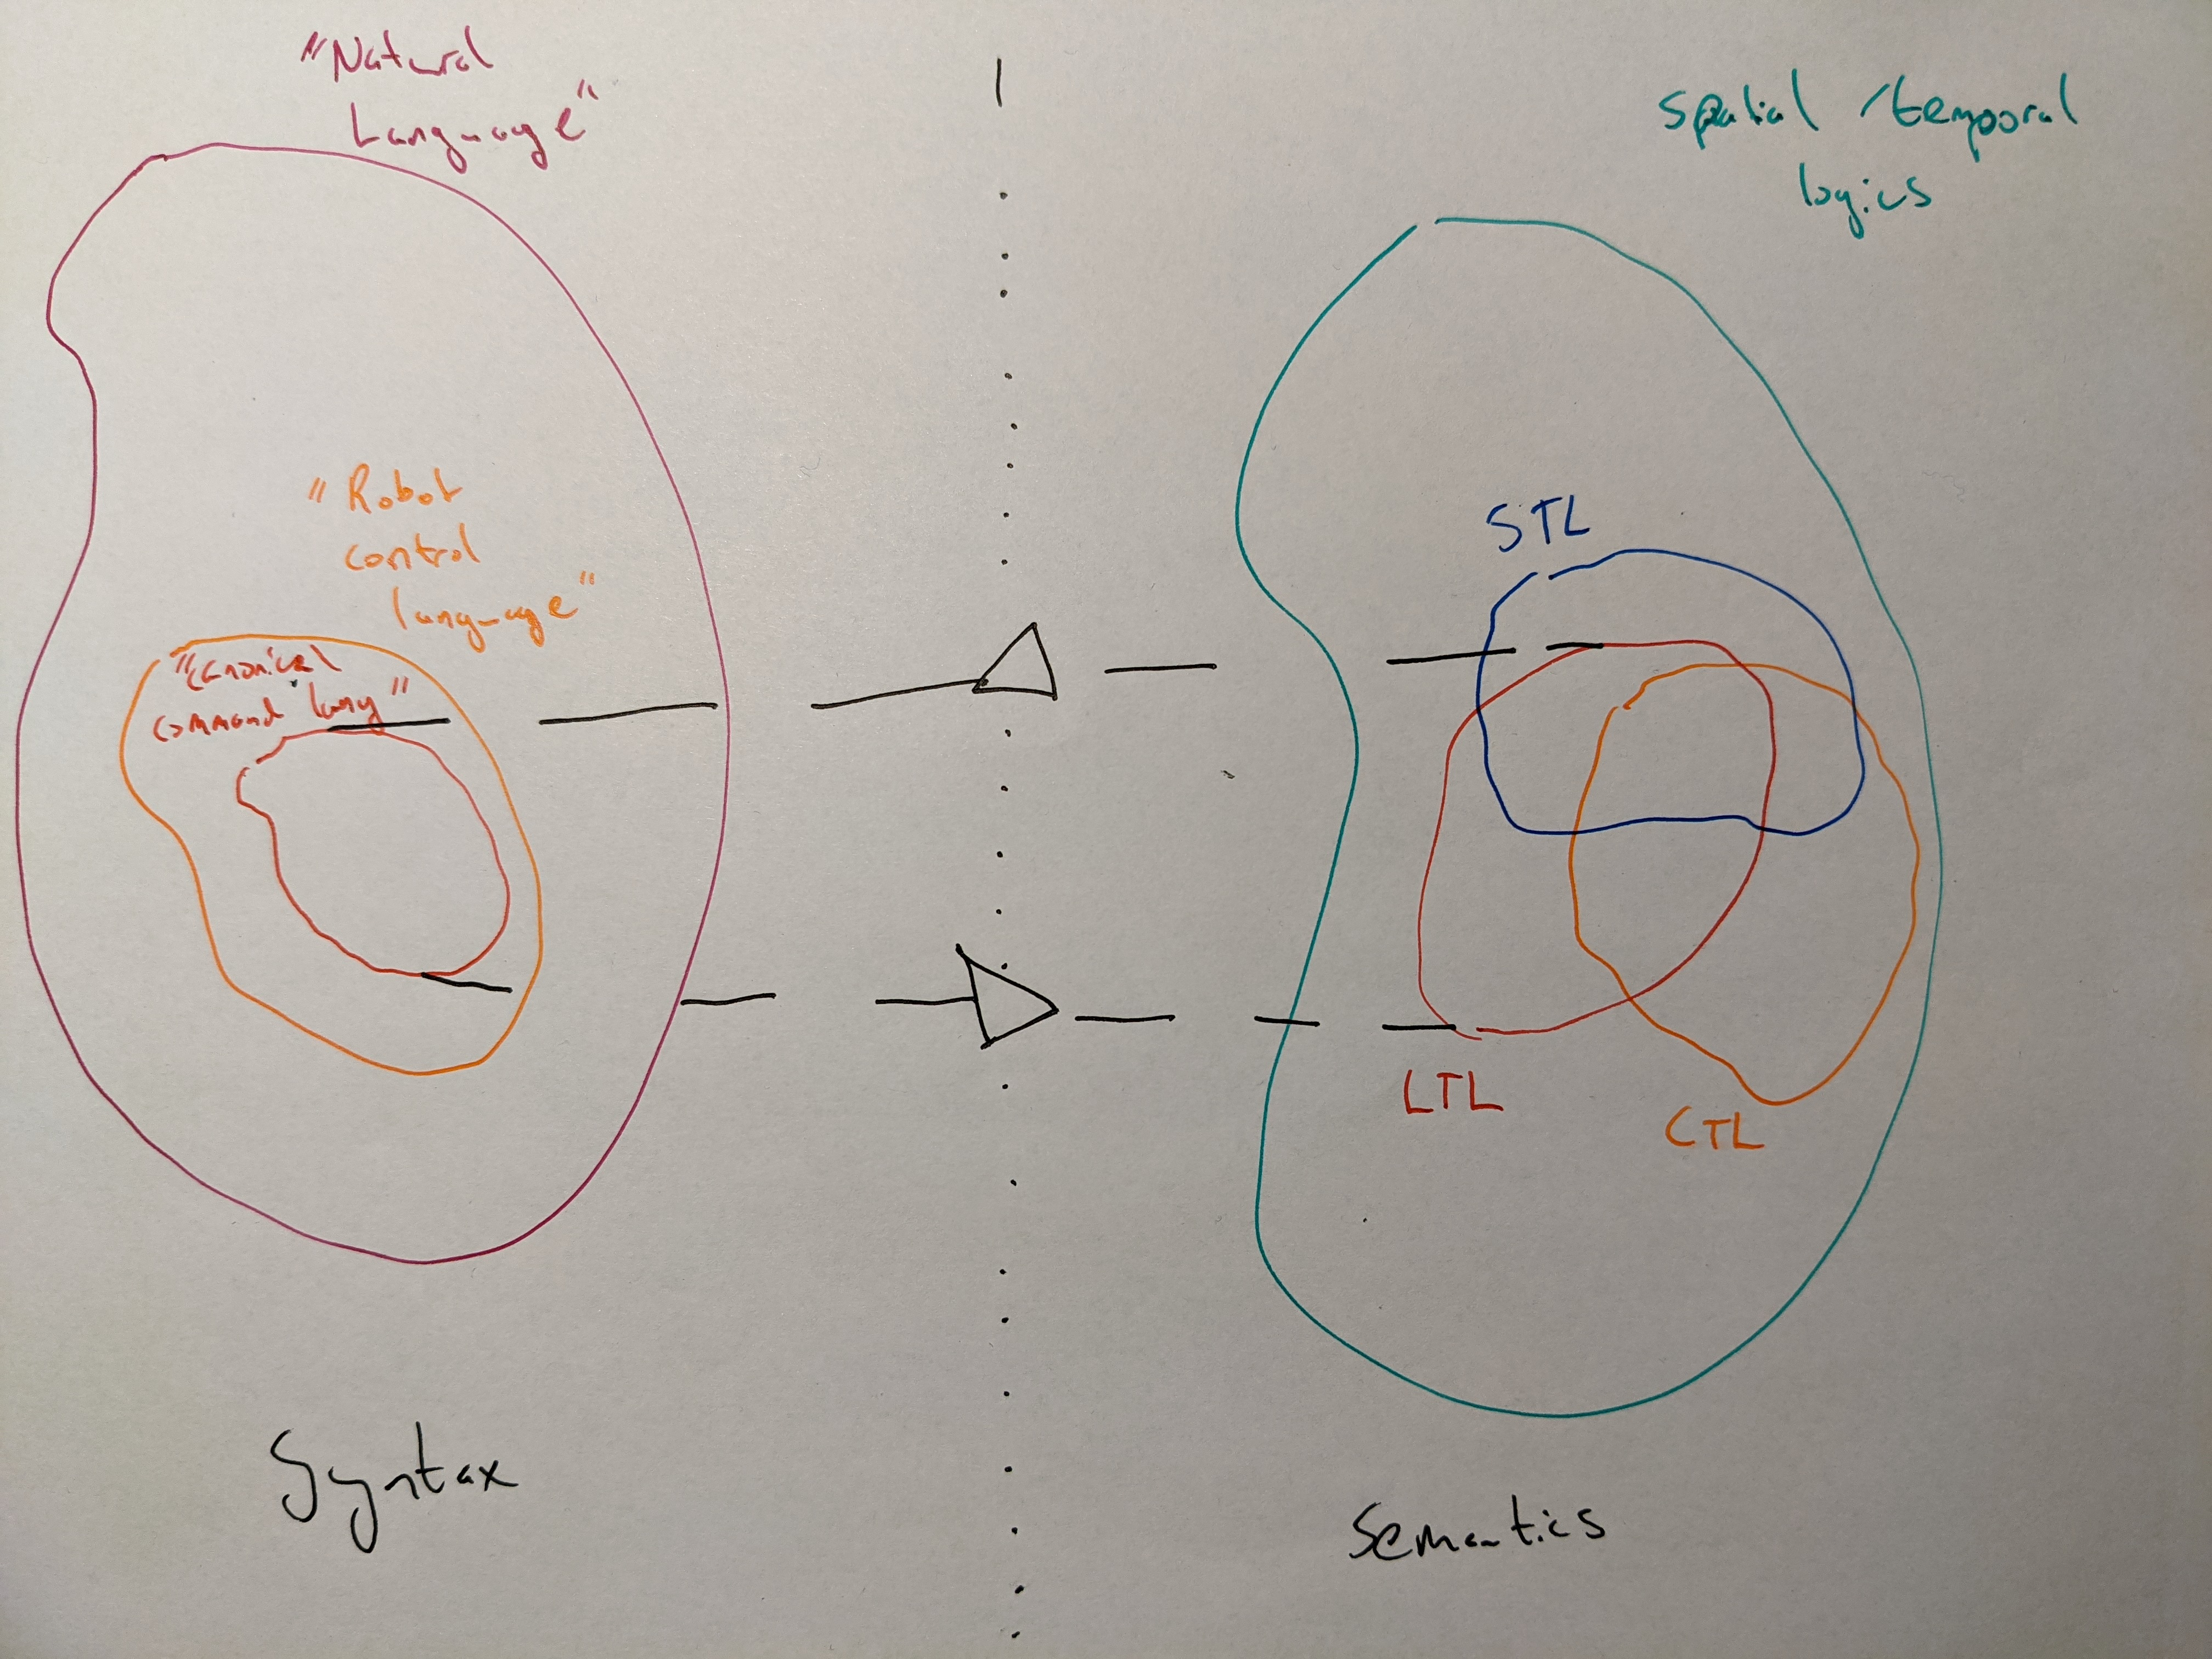
\includegraphics[width=150mm]{pics/one.jpg}
\caption{Language and Logical Spaces of Concern} \label{fig:M1}
\end{figure}

We begin in \autoref{fig:M1} with a high level overview of this semantic parsing
system, whereby the space of natural language syntax can be mapped to some
formal language semantic space (and possibly have some kind of inverse mapping).
We note that ``Natural Language'', while an idealized notion, can be thought of
the space of interpretable utterances. The relatively small subset of these
utterances which one might give to a robot, labeled ``Robot Control Language'',
is the ideal breadth our system would support, is still actually very large. We
therefore applying another filter, to the ``Canonical Command Language'' which
is inductively defined via some relatively thin set of grammar rules, which
simultaneously generate and parse expressions in some logic. Although we target
LTL because of its prominence in the literature and relatively straightforward
implementation and interpretation, it should be noted that their are other
temporal logics which may well be more expressive and better suited to the
actual problem of synthesizing controllers.

\begin{figure}
\centering
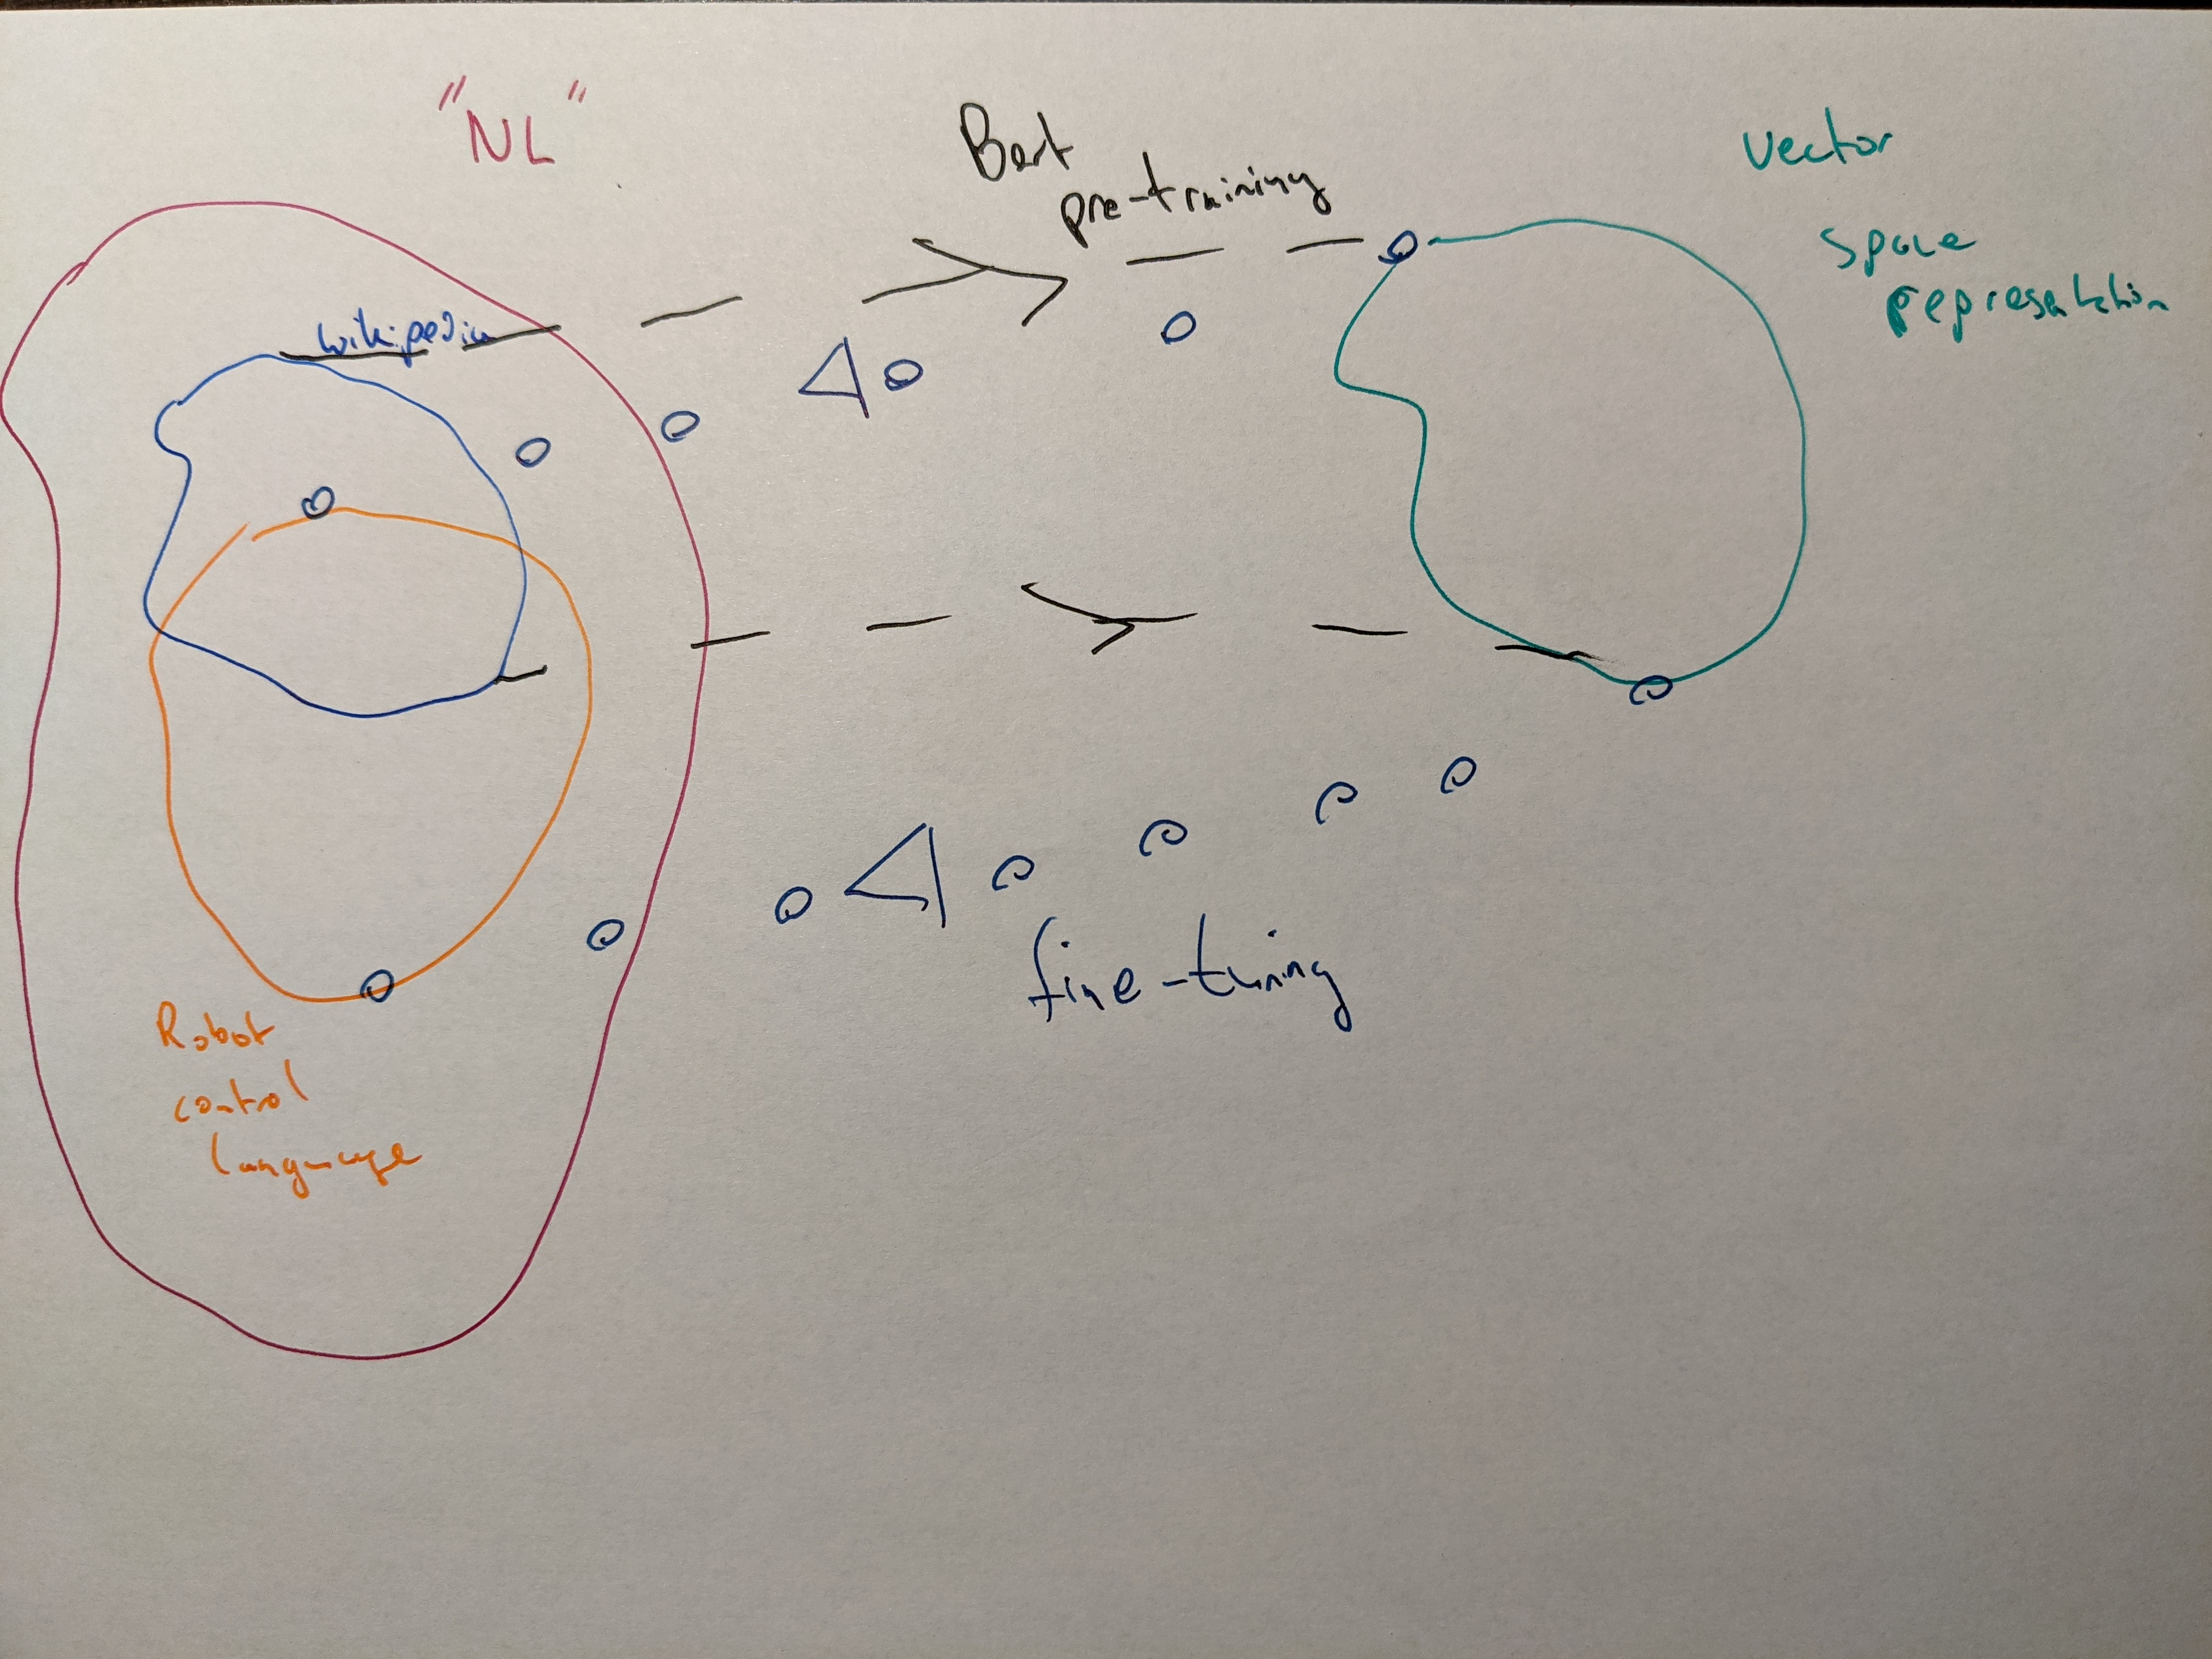
\includegraphics[width=150mm]{pics/two.jpg}
\caption{Transformer to Robot Control Language}\label{fig:M2}
\end{figure}

Due to the recent influx of transformer based language models like Bert and
GPT-3, we take for granted that the easiest way to target our ``Robot Control
Language'' will be through fine-tuning one of these models, as shown in
\autoref{fig:M2}. These transformers, trained on a separate corpus like
Wikepdia, can be mapped to some suitable set of robot commands, even though
these types of expressions will have a sparse presence in the corpus the model
was initially trained on (presumably Marco will know more about this than me).

In this context, we can then further refine the language to something less
natural, but more well-behaved. The whole proposed pipeline in \autoref{fig:M3},
indicates using the methodology as used in \cite{fewShotSem}, whereby the
semantic parser should ideally be able to take any command from the Robot
Control Language and turn it into a set of temporal logic formulas, distributed
according to most likely interpretation.

Ideally, the downstream dialogue system should either be able to ask for
clarification if two formulas are determined to be of some relative likelihood,
reject a formula that is not determined to be achievable (for whatever reason),
or synthesize a sequence of actions (and express those in the CNL) according to
the possibly modified current path.

\begin{figure}
\centering
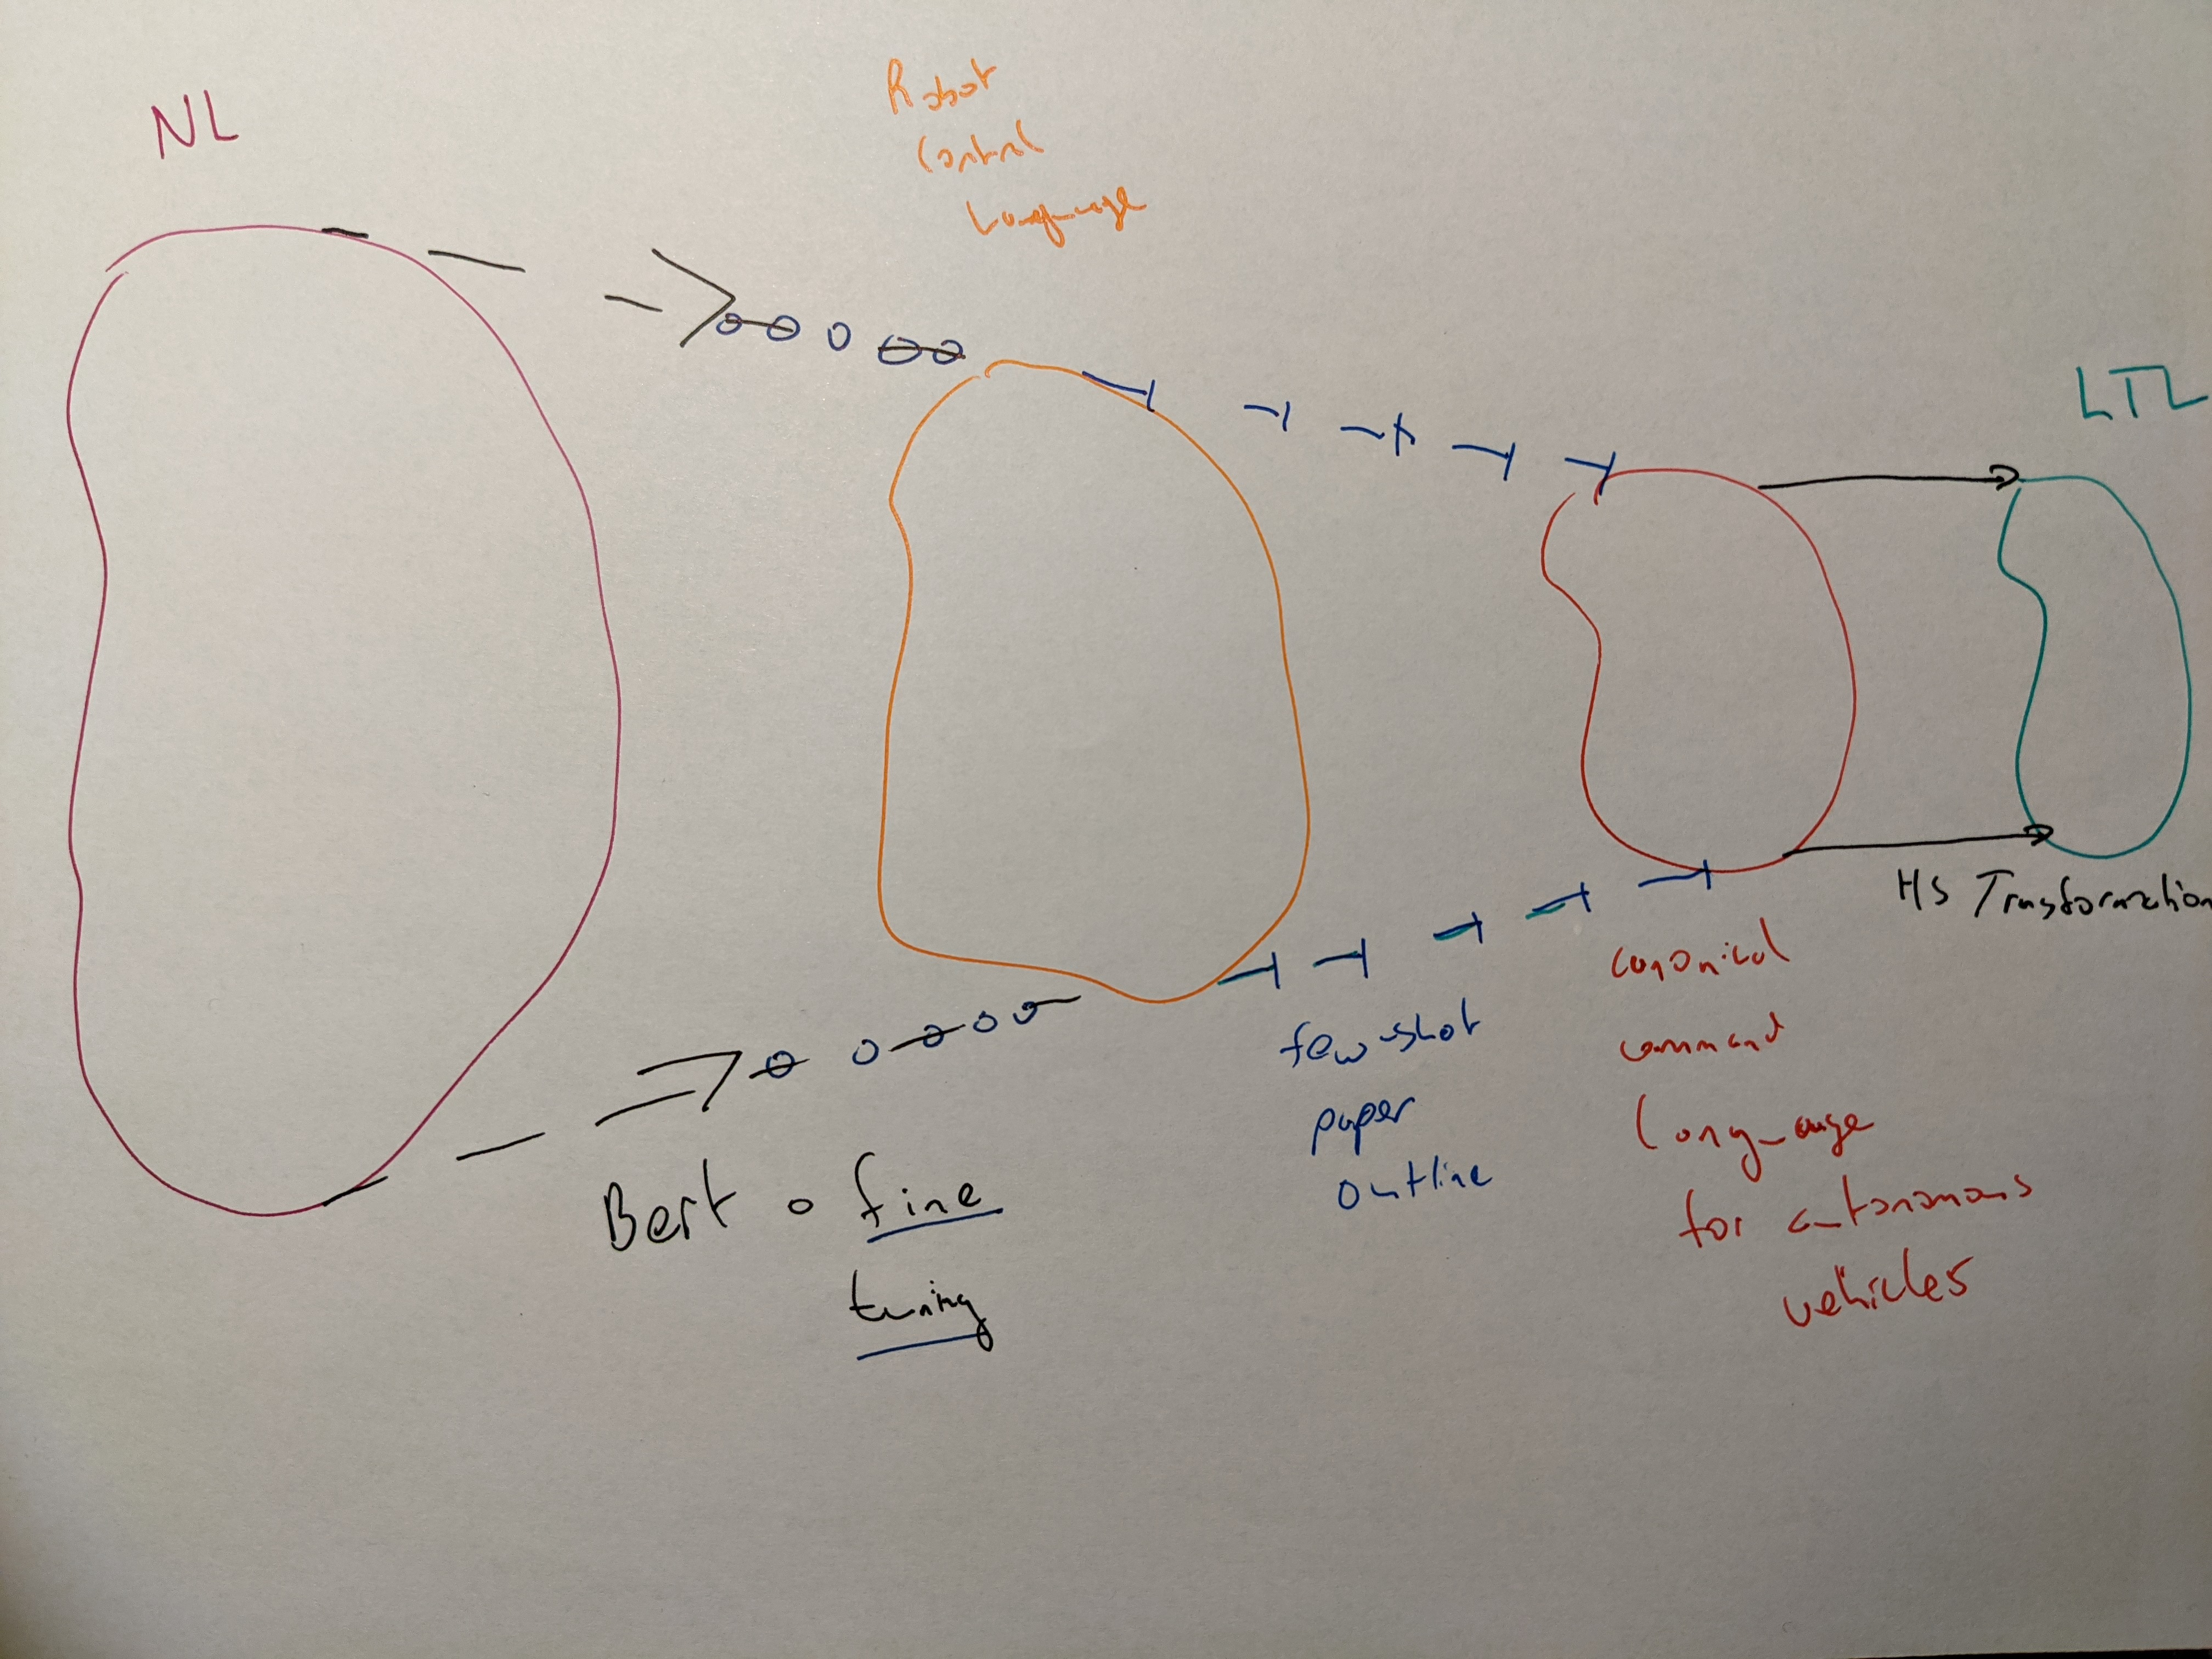
\includegraphics[width=150mm]{pics/three.jpg}
\caption{Pipeline from NL to LTL}\label{fig:M3}
\end{figure}

In theory, we can embed clauses which in turn reflect all of natural language :
``Stop at the man who is watching the tv show on his phone about time traveler
who goes back to the 12th century Mongolia, whereby the man, not speaking
Mongolian ...'' This is clearly outside the boundary of what the robot control
language should support, and ideally would be accepted or rejected by the
computer prior to the commands completion depending if there was a man looking
at a phone. Our parser currently accepts strings in our primitive canonical
language, designed in Grammatical Framework (GF), such as :

\begin{verbatim}
  p "drive to the store , turn right and stop at the dog"

  MultipleRoutes And (ConsPosCommand (SimpleCom (ModAction Drive (MkAdvPh To
  (WhichObject The Store)))) (BasePosCommand (SimpleCom (ModAction Turn
  (WherePhrase Right))) (SimpleCom (ModAction Stop (MkAdvPh At (WhichObject The
  Dog))))))
\end{verbatim}

However, we may envision our system being able to accept an expression in the
Robot Control Language like ``hit the petal till we reach the store, hang a
right, and halt when you see a cute little puppy''. We could certainly adjust
our parser to accomodate this, but it would be one of many possible edge cases
unlikely to be uttered. To accomodate many more such edge cases would cause an
exponential blowup in the parser size (thereby slowing down parsing), but more
importantly, cause the programmer a headache in building the parser, and then
mapping the NL ASTs to a LTL form. If we treat $F$ as the operating
expressing the existence a future state, $X$ as the next state, and $G$ meaning
the universal future, our desired LTL formula would most likely treat this as
$F\ (store \land\ (X\ turn\_right\ \land\ (F\ (G\ dog))))$, although we propose
that the actual grounding of these to images or controllable actions to some
downstream system.

LTL has been a popular logic for specifying controllable robot behaviors,
particularly with respect to verification of their behaviors. In
\cite{verifiedMotion}, Rizaldi et al. prove logical correctness of a motion
planner with respect to LTL formulas over maneuver automata formulas in the
Isabelle/HOL theorem prover, a non-dependent cousin of Agda. We are choosing to
deeply embed LTL in Agda for a few reasons, although the syntax of the embedding
could easily be translated to any other dependently typed theorem prover, and
with a little more effort probably any functional programming language. The
composition of a ``weakly verified'' natural language front-end with a formally
verified back-end such as in Rizaldi's work would pave the way for a fully
verified, utterance-to-vehicle-path pipeline for the autonomous vehicles.

The big question to address is what kind of verification conditions the natural
language component should be subjected to, and what kind of attacks would be
most important to preemptively anticipate. Substitution based attacks
\cite{substAttacks}, for instance, have been consistently emphasized throughout
our discussions so far. The question is, \emph{where} in the pipeline it would
be best to filter out the vulnerabilities, as well as \emph{how}.

One possibility would be to define words modulo equivalent meanings using
Wordnet \cite{wordnet} in the syntactic phase, either via training
\cite{ren-etal-2019-generating} (presumably during the fine-tuning to the Robot
Command Language or our ``canonicalization'' from that). It has been suggested
that Bert is already relatively robust against such attacks
\cite{hauser2021bert}, but we nonetheless feel that even higher sensitivities of
robustness may be better done at other phases in the pipeline.

Alternatively, one could just map these equivalent Wordnet forms to equivalent
parse trees using the Portable Grammar Format (PGF) Haskell library, which
essentially deeply embeds a GF grammar into a Generalized Algebraic Datatype
(GADT).

For instance, if we abstract over all abstract syntax trees for our grammar
using this library, we can define the following Haskell functions to equate a
``female human'' with a ``woman''. 

\begin{verbatim}
treeMapfemalePersonIsWoman :: forall a. Tree a -> Tree a
treeMapfemalePersonIsWoman (GModObj GFemale GPerson) = GWoman
treeMapfemalePersonIsWoman GWoman                    = (GModObj GFemale GPerson)
treeMapfemalePersonIsWoman gp = composOp treeMapfemalePersonIsWoman gp
\end{verbatim}

There has been work integrating multiple language Wordnets with GF
\cite{virk2014developing}, so it would presumably be easy to integrate with our
system, depending on how large we want the grammar to get.


As it is unclear what the best direction for this is, and how the attacker model
in the context of an autonomous vehicle might work, all these decisions need to
be made in the context of discussions within the group.

[ Addendum before meeting : ]

The TOUCHDOWN data set \cite{chen2019touchdown} seems like the most
comprehensive and relevant data we'll find to fine-tune via one of these
pre-trained models. Please see https://github.com/lil-lab/touchdown


The idea of domain specific pre-training can be traced to
\cite{gururangan-etal-2020-dont}, where the authors introduce the concepts of
\emph{domain-adpative pretraining} and \emph{task-adpative pretraining}, whereby
this additional pre-training phase greatly improves efficacy of the LM on
corpus and task data not well represented in the training data.

The language models have been show \cite{bioBert}

\subsection{Data Set}

The most comprehensive data set known to us is the TOUCHDOWN data set
\cite{chen2019touchdown}, which can simultaneously serve as a data source to
inform the actual grammar (ideally, we'd like to be able to generate a grammar
from a data source)

authors use ``interactive visual navigation environment based on Google Street
View''

position of the agent relative to an object, and the position of two objects
relative to one another
``resolving the spatial descriptions'', but we focus only on the navigation part
of the task

Positive

\begin{itemize}
\item Real-world observations
\item Real descriptions of these observations
\item Diverse, relatively large
\item
\end{itemize}

Follows ``instruction writing, target propagation to panoramas, validation, and
workers and qualification'', the validation here 

That having the data grounded is both incredibly beneficial, but also makes
designing the syntax and semantics tricky.

\begin{itemize}
\item Finding the touchdown only coarsely approximates general navigating in a city.
\item The workers
  aren't in a place they know, so everything the reference is in their immediate
  visual environment
\item and this is a ``short-term'' task, it requires no long-distance navigation
  and reasoning 
\item Limited to NYC, hectic urban environments (also, daytime)
\item Working with panoramas is not necessarily a great simulation to a real environment
\item ``They are not per- mitted to write instructions that refer to text in the
images, including street names, store names, or numbers''
\item No temporal reasoning (as spatio-temporal is assumed)
\end{itemize}

Ideally our data set would then have the properties

\begin{itemize}
\item Long and short-term tasks
\item Different cities, different languages (this will be dependent on the
  context of the data collected), for instance, where there are dirt roads
\item Updates over time (the user can update a context locally or globally) on
  the road
\item Users with various degrees of contextual information
  Contextual information
  - street place, names (named entity recognition) accessible to google
  - people's names (mom's house)
\end{itemize}

That the data collection task in an objective way is inherently tied to the way we approximate it in
collecting data, thereby limited by our experimental apparatus and assumptions
in designing the data set.

What is the actual feasibility of this stuff?

how well does a given logic allow us to reason about a space of instructions.
What is the logic grounded to, how it is verified , all of these may effect the
choice of formulas

we can't just design a perfect language to capture our meaning - goes back to
the wishful thinking of Frege, but we can try to approximate it

next intersection (and next left?) versus next gas station versus ``next to''
 will be a store on your left with stars next to the name.

there is could either be 
``all of the apartment buildings on your left''

if you are going the correct way.
logical content
You will know you're on the correct road if to your left there are planters in the middle of the street


\subsection{Syntax and Semantics}

When designing a grammar, we can pretend that initially

san abstract syntax, we have the following considerations

That when we are conditioning our syntacitc model of emperical, noisy, and
biased natural language data, so as to ideally generalize to unencountered
phenomena.

A central insight ambiguity : 


\begin{itemize}
\item Ontological semantic space. What are we trying to represent?
\item Intended semantic space, the logical or formal system which our grammar
  will map to (via Haskell transformations)
\item  We want to account for some grammatical constructions via the abstract syntax, but
  outsource most of the grammaticality to the RGL
\item Data source. How to conform to the data set in a way that's faithful but
  doesn't overfit (the overfitting can probably result in generating functions
  which are useless and either make our parser slow down or overgenerate)
\end{itemize}

While theres no clear way of relating the trade-offs, we can come up with some
heuristics that shed light. Developing the ``ontological design'' allows one to
capture the intuitive problem.


\subsection{Ambiguity}

What happens when we encounter ambiguity? For instance, in p "go to the person
with the dog ." The prepositional phrase "with the dog" can either modify person
(as an adjectival clause) or it can modify go (as an adverbial clause). Because
the parser is designed to accommodate simple cases of both types of clauses,
these ambiguities, even in simple sentences from our corpus, will grow quickly. 

In the case of a vehicle, however, knowing the correct parse is dependent on
the context in which the driver is going to the person : is the language
grounded in the fact that there a dog in the car, or a person in the purview
with a dog (or, most confusingly, perhaps both conditions are met, in which case
more contextual information is required to disambiguate the correct parse).

For we can actually program the semantics to accommodate both scenarios, whereby

$F (manwithdog /\ G Finish)$
$F (man /\ G Finish) /\ G withdog$

We can define our semantics to accommodate both interpretations, whereby the
parses produce unique semantic conditions, and the LTL solver will have to see
which condition is more easily satisfied. While this edge case may seem overly
pedantic to consider, as one's intuition might suggest the first case to be
overwhelmingly more natural, the

We should just make simplifying assumptions, though, at least for the purpose of
a grammar like ours.

probably scrap
\section{Alternative ideas}

While the evaluation of machine learning systems provides assurances using
different scores and metrics on different tasks assures one they may on average
perform better than humans at certain tasks, the advent of adversarial attacks
\cite{szegedy} with the intention of deceiving such a system by a hostile actor
leads the system designer to desire, and possible require additional
verification about the system's behavior. In the context of natural language
processing (NLP), where data sources rely on strings of text, these attacks can
focus an array of features from spellings of individual words to rearranging
entire sentences \cite{}. So-called synonym attacks, which adversarially target
the system at the lexical level, can cause traditional NLP models to [...]
\cite{}.


Aside from the user experience being compromised by a system which has been
adversarially afflicted, there is also a possibility of physical danger for the
passenger and other people in the vicinity. As voice directed robots have many
possible points of failure, we focus on two types of verification for our
system. Rather than focus on breadth of language coverage, which ML language
models excel at of due to their reliance on statistical modeling and tons
of data, our system is narrowly focused as a proof-of-concept, from which it
could either be extended by hand, or different components modified using
other techniques and tools.



\printbibliography


\end{document}


% LocalWords:  CNLs
